% !TEX root = ../main_standard.tex
\chapter{Literature Review}
In this chapter, previous research and techniques relevant to the
project are reviewed. The first part of the chapter basically describes
the general animation techniques such as key frame animation,
procedural animation, kinematic animation and physical animation. The
fundamentals of animation such as how to represent an object and
manipulate these objects are also included in this part. The second
part mainly focus on rendering techniques and animation techniques
specifically for the arthropods.

\section{Attributes of a spider}



\section{Representing an object} 
There are many alternative representations of an object in computer graphics, such as polygons, parametric patches, constructive solid geometry, etc. Among these representations, the most popular method is using polygonal facets, usually a mesh of triangles which referred as a Boundary representation \cite{alan3D}.This section will discuss how to use polygon meshes to represent an object and how to manipulate them. There are three subsections in this section. In the first subsection, a simple cube model using face-vertex will be introduced. The second subsection will generally describe the control techniques(rigging and skinning) for more complex mesh models such as a human model. In the final subsection, a robot model made of basic geometric shapes such as sphere and cylinder will be built with the help of scene graph. How to manipulate the robots into different postures with scene graph will also be included in this subsection. 

\subsection{A simple mesh model} 
Polygon meshes also could be represented in various ways by using different methods to store the vertex, edge and data. 
One most widely used is face-vertex meshes\cite{facevertex}.
In face-vertex meshes, an object is represented as a set of faces and
a set of vertices. Face-vertex meshes allow both explicit lookup of
the vertices of a face and the faces surrounding a vertex. Figure
\ref{fig:graph1} is a cube example as a face-vertex mesh. Since in
this example, every face is represented in a triangle, each face has
exactly three vertices. However, it is easily seen that not every
vertex has same number of faces(e.g., v0 has 5 faces, v8 has 4
faces). 
\begin{figure}[ht!]
\centering
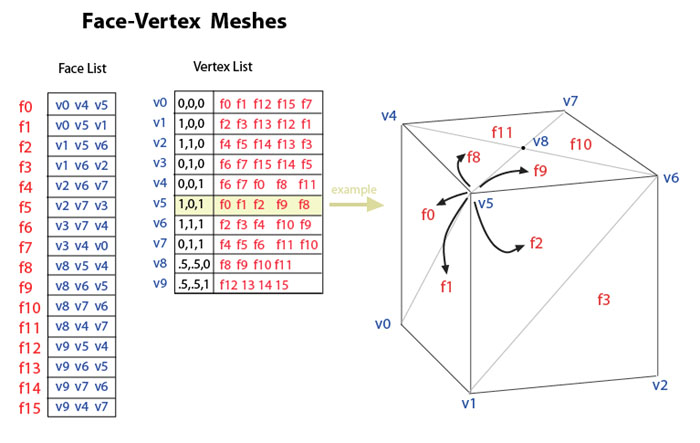
\includegraphics[width=13cm]{figures/figure1.jpg}
\caption{Face-Vertex Meshes \protect\cite{fv}}
\label{fig:graph1}
\end{figure}
The advantages of face-vertex meshes is that it is easy to traverse all structures. Moreover, locating neighboring faces and vertices is constant time because both faces and vertices are explicit. However, it is not same case for locating face given another face because the edge information is implicit. In rendering process, the face list usually transmitted into the GPU as a set of indices and each vertex usually contain three properties: position, normal and color. The advantage of this is when the shape is changed, only the vertex data need resending without updating the face connectivity.
Despite the popularity and simplicity of polygon meshes, there are difficulties in changing the shape in animation. First, moving polygon mesh vertices will disrupt the where a shape has been converted into polygons with some degree of accuracy. Second, altering a large part of an object which may involve moving many elements at the same time. Third, the level of details should also be considered when rendering from different distances \cite{alan3D}. 
\subsection{A complex surface mesh model}
The left part of figure \ref{fig:rigging} is a complex human mesh model. It is easier to manipulate the complex mesh model in a hierarchical structure.
\begin{figure}[ht!]
\centering
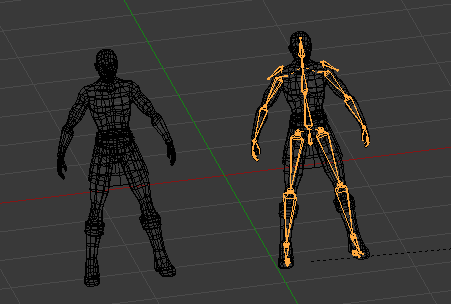
\includegraphics[height=8cm]{figures/rigging.png}
\caption{A complex human mesh and rigging \protect\cite{shaolinpic}}
\label{fig:rigging}
\end{figure}
Usually to animate or pose a complex articulated structure, a set of
bones or skeletons are added such as the right part in figure \ref{fig:rigging}.  As a result, when we want to make the angle between 
upper arm and lower arm as 60 degrees, we could make the angle of the bones as 60 degrees.
This process is called rigging which
usually includes linking the bones in a hierarchy,
setting constraints on the bones' movement(usually degrees of freedom
of the joints), and set up controls such
as inverse kinematics and forward kinematics.
There are also many automatic rigging techniques which saves lots of
artists' time. \cite{Rigging1} implemented a system can automatically rig and skin, in which the main method adopted is to calculate the bone iteratively based on assuption of weight-like parameters.  \cite{Rigging2}  implemented a more advanced system by adopting an example-based rigging approach where the skeleton is more compatible with most existing popular animation software.
\subsubsection{Skinning}
Skinning is to bind a skin to the skeleton which means that every
vertex of the continuous skin mesh is attached to a joint. As a
result, the skin vertices are moved when the skeleton is moved.
A basic skinning approach is rigid skinning where the relative
position of the vertex in the local joint frame does not change. It is simple but has the disadvantage
of large distortions at bends. Vertex blending is another approach
which tackles this problem but has the skin collapse problem
\cite{skinning1}. \cite{skinning2} implemented an approach which could
automatically skin deformable mesh animations with no need for
specifying skeletons.
\subsection{A complex object built from pieces}
An alternative way to build an object is to use pieces rather than a single complex mesh. As an example, we will consider building a robot from pieces. The most obvious way to do it is directly put the
pieces in certain position. However, problems come when we want to make
the robot pose in certain gestures. Because it is hard to calculate the
final position and orientation of some parts of it such as the finger
of the robot. It will be
much more simple if the relationship of different parts could be
taken into consideration(e.g., when the arm rotates around shoulder,
the finger will translate and rotate accordingly). 
A scene graph is a general data structure which arranges the logical representation of a
graphical scene. 
It is usually represented in a collection of nodes in
a graph or tree structure. It also could be used to structure the parts of a complex object made of pieces. For example, Figure \ref{fig:graph3}  is a simple robot example and
its scene graph.  The nodes can also be grouped into a compound object(e.g. the left shoulder and
all its child could be grouped as left arm.) that can be
transformed, selected, etc. as easily as a single object.   
An operation on a parent node automatically
propagates its effect to all its child nodes. If the upper arm rotates around the shoulder, all its
child nodes(e.g., elbow, lower arm etc.) will be affected. Figure
\ref{fig:scenegraph2} is the robot and its scene graph after adding two
rotation R1 and R2. It is easily seen the advantages that only by
rotating the two upper arms around their shoulders, all its child
nodes such as elbow, lower arms, palm and fingers will move
automatically without specific transformations on these nodes.
\begin{figure}[ht!]
\centering
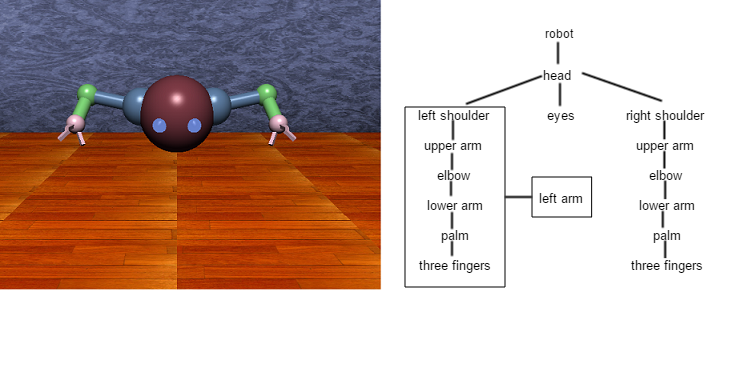
\includegraphics[width=12cm,height=5cm]{figures/figure3.png}
\caption{A simple Robot and its scene graph.}
\label{fig:graph3}
\end{figure}
\begin{figure}[ht!]
\centering
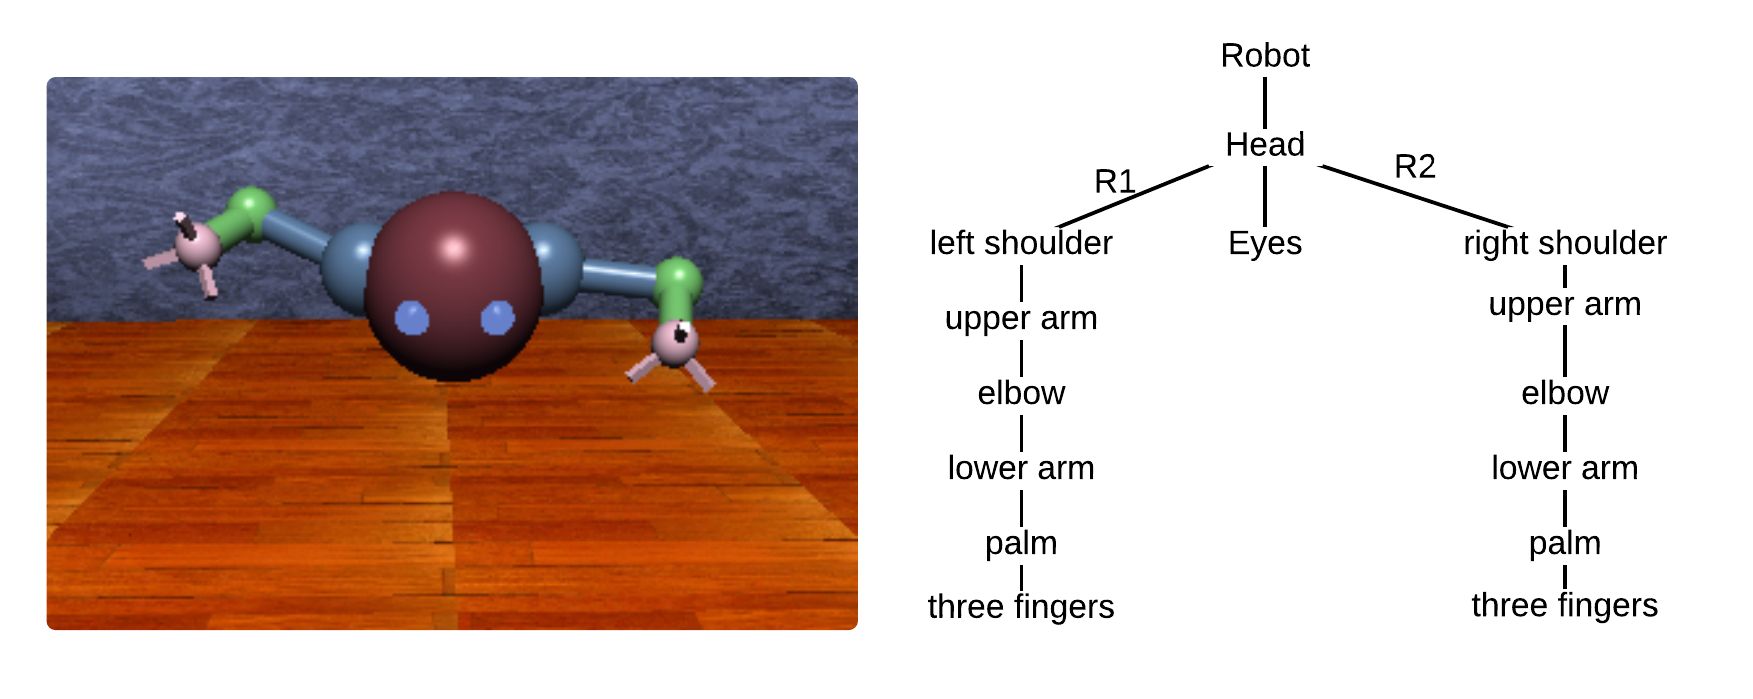
\includegraphics[width=12cm,height=5cm]{figures/scenegraph2.png}
\caption{A simple Robot and its scene graph after transformation.}
\label{fig:scenegraph2}
\end{figure}
Scene graphs can also combine bounding volume hierarchies, spatial
partitioning and many other techniques. There are also a lot commercial
software and 3D graphics libraries that use a scene graph such as Unity 3D and
Java 3D.
\section {Spider Animation}
Animation could be divided into three categories: low-level, medium-level and high-level approach\cite{alan3D}. In the low-level approach, a geometric description is given such as the position and orientation. A typical example is keyframe animation.  In the medium-level approach, an animator has to input some rules which could be borrowed from real life or exactly physical rules instead of inputing the details of the geometric description. Usually an animator could know the rough results but no details of how the animation could be in this kind animation. To get the exact results, an animator has to run the simulation and adjust the rules for lots of times. Procedural animation and physical animation could be fell into this category. The high-level approach is behavioral animation.\cite{animationSlides} It will be performed by the coeffect of the environment setup and the animation internal system. The action selection layer in \cite{steering} is an example. In sum, the advantages of lower level approach is that it has more control abilities than higher level approach, but it will need lots of mannual efforts and sometimes it is infeasible to be implemented.
 
\subsection{Keyframe Animation}
In key frame animation, first the attributes of an object such as orientation, the position and joint angles between the links are at set at certain instances. Then interpolation of these attributes between these instances will be done. For example, A sequence of robot movement could be seen in figure \ref{fig:movingRobot}. Here for example first we set the attributes of the robot in \ref{fig:movingRobot-a}. Then also set the attributes of the robot in figure \ref{fig:movingRobot-d}. Then the interpolation of the position of the robot is a half circle linearly in x time. The interpolation of the orientation is 180 degree also in x time linearly. Then in-between pictures such as the pictures of figure \ref{fig:movingRobot-b} and figure \ref{fig:movingRobot-c} will be generated automatically. This idea was originated from Baecker's Genesys Computer Animation System in which the animator had to input
parameters of curves to specify both the path and timings of the 2D
animation \cite{keyframe1}. 
\begin{figure}
\centering
\subfloat[Part 1][]{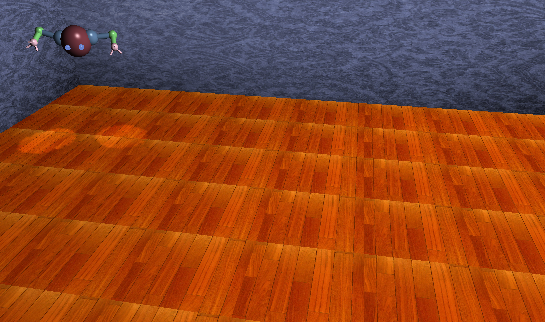
\includegraphics[width=2.5in,height=1.5in]{figures/rb1.png} \label{fig:movingRobot-a}}
\subfloat[Part 2][]{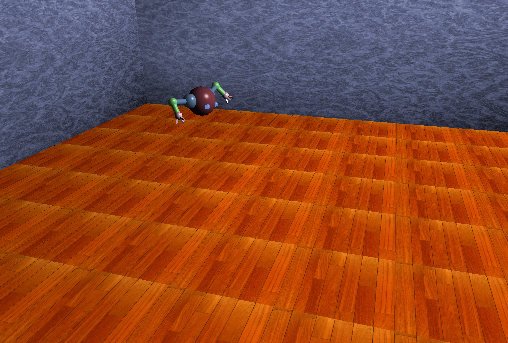
\includegraphics[width=2.5in,height=1.5in]{figures/rb2.png} \label{fig:movingRobot-b}}\\
\subfloat[Part 3][]{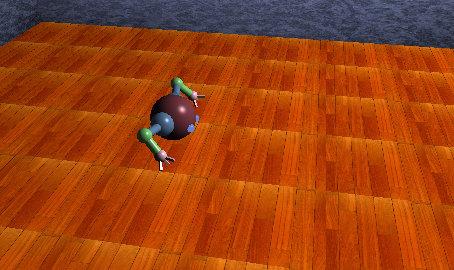
\includegraphics[width=2.5in,height=1.5in]{figures/rb3.png} \label{fig:movingRobot-c}}
\subfloat[Part 4][]{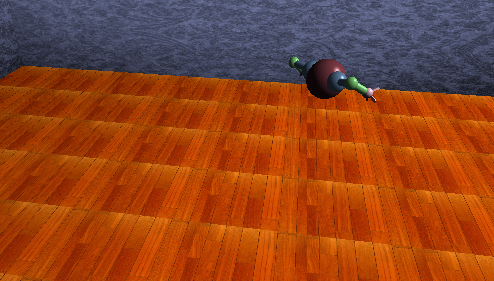
\includegraphics[width=2.5in,height=1.5in]{figures/rb4.png} \label{fig:movingRobot-d}}
\caption{A moving robot.}
\label{fig:movingRobot}
\end{figure}
Except these attributes, the shape can also be interpolated shown in figure \ref{fig:cows}. It is obvious that the number of the vertices of different pictures are different. One issue in shape interpolation is to tackle the relationship of corresponding vertices when the number is changing. The relevant research could be found in \cite{2d_shape}. 
\begin{figure}[ht!]
\centering
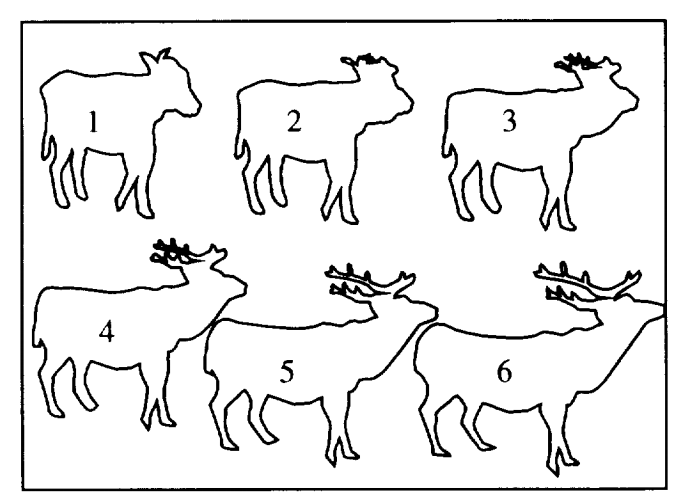
\includegraphics[height=8cm]{figures/cows.png}
\caption{Shape interpolation of a cow.\protect\cite{2d_shape}}
\label{fig:cows}
\end{figure}
Recent research combines the
data driven approach solves this problem \cite{keyframe2}, \cite{keyframe3}.  However, due to the
essence of the keyframe animation, even with data driven approaches
can not produce very substantial and dextrous animation for small
objects with an acceptable amount of data. Additionally, although \cite{keyframe4}
had implemented a system for capturing the motion data of insects, it
has several limits such as the system can only capture data from
planar geometry and only locomotion data is captured. Even if these problems are tackled someway, it is still has two drawbacks: production cost and lack of controllability. The problem lies in the traditional keyframe animation
is that the realism of the final motion heavily depends on the
knowledge and skills of the animator\cite{vince3D}. 
\subsection{Procedural animation}
Procedural animation refers to generation of motion based on procedures usually a set of rules other than pre-recorded data. Similar to keyframe animation, the procedural also has initial values and formulas to control how these values will be changed. But the difference is that in keyframe animation the initial values are specific attributes to show how the object is presented in an animation and the formula is about interpolation. While in procedural animation, the initial values contain some abstract attributes such as velocity and the formula show how these abstract values are changed which could be the forces which alter the velocity. It is infeasible to get the specific attributes such as position, orientation of an object in procedural animation. Examples of this kind animation could be seen in particle systems, plant growth, waterscapes, etc \cite{vince3D}.
Figure \ref{fig:mario} is a snapshot from the classic game Mario. It is a very simple form of procedural animation. When a key is pressed, acceleration is added to the velocity where the direction is the same as the key pressed. In this example, the procedure is a combination of responsive effects which is to add the acceleration in the same direction as the key pressed and deceleration in the reverse direction of the velocity. 
\begin{figure}[ht!]
\centering
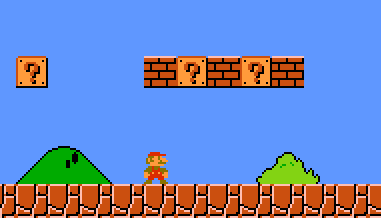
\includegraphics[height=6cm]{figures/mario.png}
\caption{A snapshot from classic game SuperMario}
\label{fig:mario}
\end{figure}
 Procedural animation is also widely developed is procedural
locomotion.\cite{loco1} implemented an interactive hierarchical motion control
system by using inverse kinematics with optimal approaches which
generate human walking over uneven terrain in different
environments. \cite{loco2} reviewed three categories of human walking which
includes procedural methods based on knowledge-based kinematic
animation.
\subsection{Kinematic animation}
The kinematics originally comes from the robotics which is intended to solve the relation between the joint angles and end-effector 
of an articulated figure. There are two categories in kinematic animation: forward kinematics and inverse kinematics. The forward kinematics is given all the joint angles to calculate the end effector X. The inverse kinematics is given the end effector X to calculate all the joint angles which produces the position of the end effector X.\cite{alan3D}
\subsubsection{Forward Kinematics}
Forward kinematics could be seen as a special kind of scene graph. In the graph, every node except leaf node is specification about the angles of joints while the leaf node contains the information of the end effector X. Thus every time a joint angle changes, it propagates the effects to all its descendant joints. As a result, the effector X will change. The advantages of it than keyframe animation is that the animator does not have to think all the attributes of a frame. Instead the animator could focus on the relation between linked parts.
So for example, to animate a human walking in figure \ref{fig:leg}. The animator just need to think the starting point of the root node of the hierarchy and angles between linked parts from the top node of the scene graph which is the hip to the "end effector" which is the foot. The curve in the picture is the angle between two linked parts.
\begin{figure}[ht!]
\centering
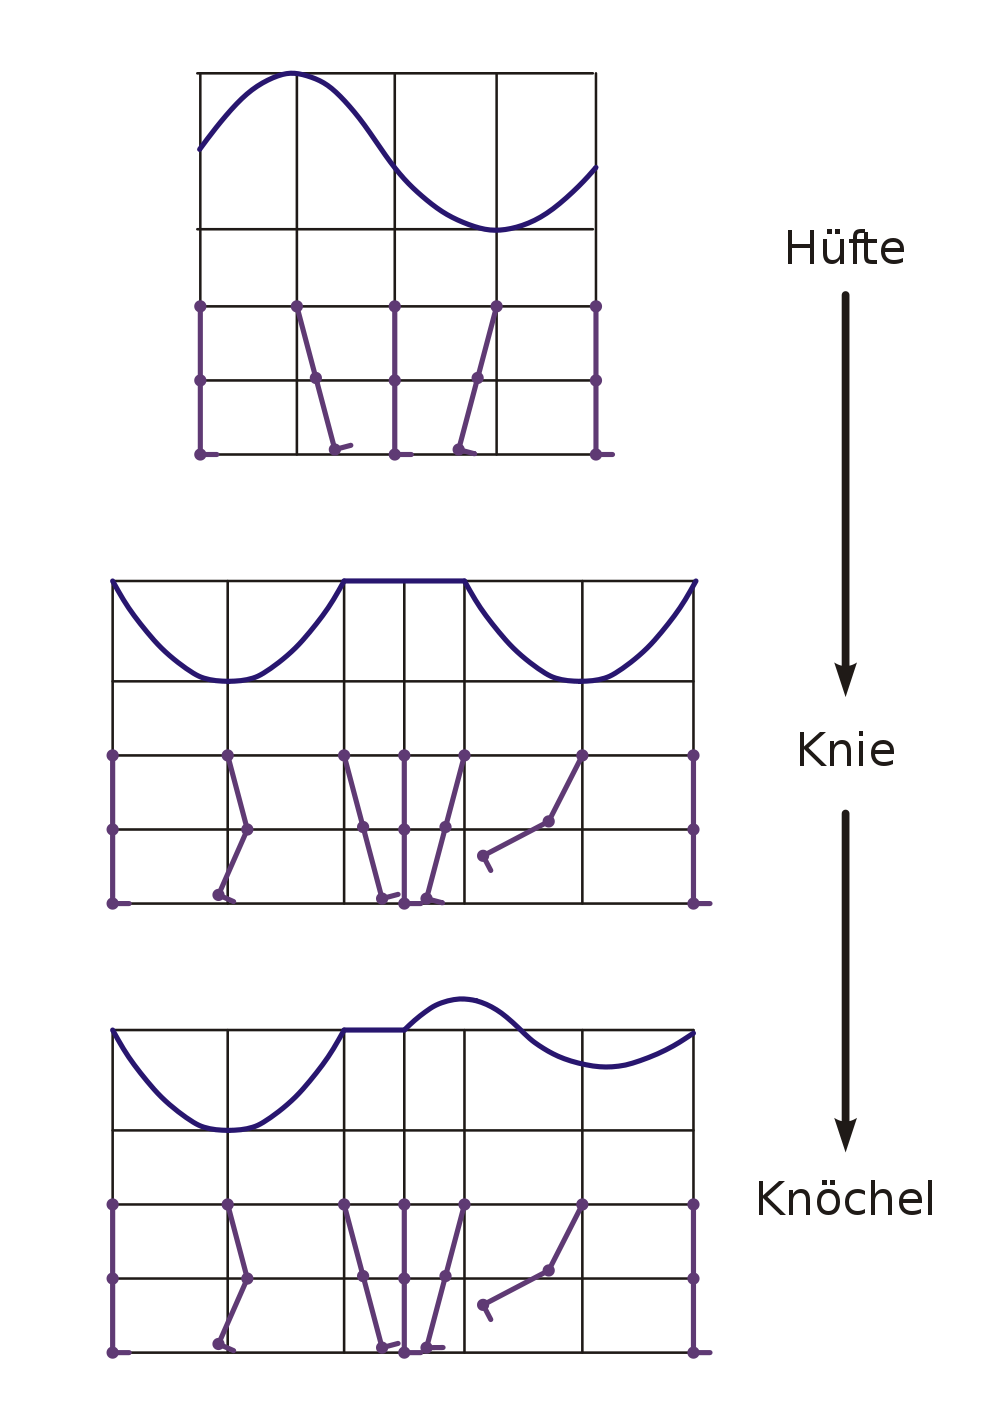
\includegraphics[width=12cm,height=5cm]{figures/leg_animation.png}
\caption{A human walking linked structure \protect\cite{leganima}}
\label{fig:leg}
\end{figure}
Since the structure could be considered as a scene graph or a hierarchy, the motion of the end
  effector is the accumulation of all the transformations that lead
  from the top of the scene graph to the "end effector"\cite{alan3D}. Given the state
  vector $\Theta{}$ which is the set of all the angles between different links in the link structure,
  the state vector $\Theta{}$ could be represented as\cite{alan3D}:
  \begin{equation}
  \Theta{}=(\theta_1,...,\theta_n)  
  \end{equation}
Because the object is a linked rigid structure which means given the starting point of the root node, each part of the structure including the end effector could be calculated by the state vector. Thus the position of the end effector \textbf{X} could be represented as\cite{alan3D}:
\begin{equation}
\mathbf{X} = f(\Theta)        
\end{equation}
So for example in a two link structure as shown in figure \ref{fig:twolink} , the end effector position is\cite{alan3D}:
\begin{equation}
\label{eq:1}
\mathbf{X}=(l_1\cos\theta_1+l_2\cos(\theta_1+\theta_2),l_1\sin\theta_1+l_2\sin(\theta_1+\theta_2))  
\end{equation}
\begin{figure}[ht!]
\centering
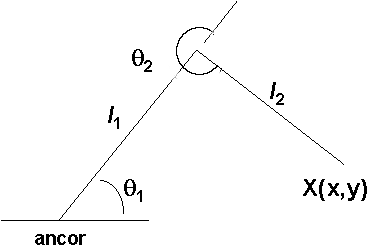
\includegraphics[height=5 cm]{figures/twolink.png}
\caption{A two link structure \protect\cite{linkpic}}
\label{fig:twolink}
\end{figure}
From the example, it is easily seen that it is more convenient than key frame animation. And constraints of angles between links could also be easily embedded. However, it is tedious to make the animation natural or as planned. Because the animator usually need to set the parameters from the top hierarchy to the bottom. If the link structures are complex, it is hard to make the end effector in the trajectory as planned\cite{alan3D}. This problem could be solved by inverse kinematics.
\subsubsection{Inverse Kinematics}
Inverse kinematics is the reverse of the forward kinematics. Unlike the forward kinematics tackle the animation problem from the top of the hierarchy to the bottom. It will first focus on the bottom of the hierarchy which is the end effector. So given the end effector X, all the parameters should be set explicitly in forward kinematics could be calculated by inverse kinematics\cite{Reference2}. Thus the problem could be summarized in an equation where given the end effector position\textbf{X}, calculate the state vector $\Theta{}$\cite{alan3D}:
\begin{equation}
\label{eq:2}
\Theta{}= f'(\mathbf{X})    
\end{equation}
Since the equation \ref{eq:2} is not linear and if the link structure become complex, it is very hard to invert the function. One way to solve the inverse kinematics is to linearise the problem by using Jacobian.\cite{alan3D}
\subsubsection{Jacobian}
Given $\mathbf{X}= f(\Theta)$ where $\mathbf{X}$ is of dimension n and $\Theta{}$ is of dimension m, the
Jacobian is the $n * m$ matrix of partial derivatives relating
differential changes of $\Theta$($d\Theta{}$) to differential
changes in $\mathbf{X}$ ($dx$), that is\cite{alan3D}:\\
\begin{equation}
dx/d\Theta=J(\Theta)\\
\end{equation}
By inverting the function, we get the following linear equation\cite{alan3D}:
\begin{equation}
\label{eq:3}
d\Theta=J^{-1}(\Theta)(dx) 
\end{equation}
Here iteration could be used by adding small changes dx towards the target position until the goal is reached. 
So one possible way to solve the inverse kinematics by using Jacobian could be\cite{alan3D}:
\begin{algorithm}
\begin{algorithmic} 
\REPEAT 
\STATE $dx \leftarrow$ small movement in the direction of $x$
\STATE $d\Theta \leftarrow J^{-1}(\Theta)(dx)$
\STATE $x=f(\Theta+d\Theta)$
\STATE $J \leftarrow dx/d\Theta$
\STATE $invert J$
\STATE $x \leftarrow x+dx$
\UNTIL{goal is reached}
\end{algorithmic}
\end{algorithm}
However since the equation \ref{eq:3} is an approximate way to calculate the real $\Theta$. As a result, the $dx$ in the algorithm above is not exactly the real changes of the end effector. The difference could be calculated by:
\begin{equation}
\|J(d\theta)-dx\|
\end{equation}
There are also several constraints in this approach. For example, differentiation is hard for a structure with many links. and the Jacobian may not invertible\cite{alan3D}.
\subsection{Dynamics and Physics-based animation}
In dynamic simulation, objects are modeled as masses acting under
forces and torques. The motion is produced through Newtonian
mechanics. Object motion in dynamic simulation is usually resulted
from a combination of automatic physical simulation (e.g., failing due
to gravity or floating in water due to buoyancy) and user suggested
forces (apply torque so that a moving car changes its velocity
direction) \cite{dy1}. It is an effective means to produce complex and
realistic behavior that will be impractical for kinematic
approaches. However the shortcoming of this approach is hard to
produce natural looking animation \cite{dy2}. 
There are two major approaches in physics-based animation. One is
motion synthesis approach which is similar to the combination of
inverse dynamics and kinematics. The difference is that it also takes
account of the limitations of the muscles. The main task of this
approach is to derive suitable actuator control functions which is
difficult when the muscle model is complex. The other approach is
constraint-based approach which involves constrained optimization and
inverse dynamics. 
\section{Arthropod Simulation}
An early research on arthropod simulation could be seen in \cite{arsimu1} where a
forward dynamic simulation algorithm was proposed for the coordination
of the locomotion of six-legged figure. The system has three main
procedural components: a dynamic simulator, a gait controller and
motor programs. The dynamic simulator is based on Featherstone's
Articulated Body method which uses reduced coordinates to represent
motion in a computational time linearly proportional time with N being
the numbers of degrees of freedom. The gait controller is based on five rules of
the gait behavior of many insects proposed by Wilson\cite{arsimu2}: 
\say{
\begin{enumerate}
\item A wave of protractions (forward movements of the legs relative to
the body) runs from posterior to anterior (and no leg protracts until
the one behind is placed in a supporting position). 
\item Contralateral legs of the same segment alternate in phase. 
\item Protraction time is constant.
\item Frequency varies (retraction time decreases as frequency increases). 
\item The intervals between steps of the hind leg and middle leg and between
the middle leg and foreleg are constant, while the interval between the
foreleg and hind leg steps varies inversely with frequency. 
\end{enumerate}}

The motor system is composed of stepping program which compute forces
necessary to produce steps and deliver forces to legs to forward the body.


\cite{arsimu3} developed a system which is used to study insect
walking. The system describe a simple neural network called Walknet
which is a biologically inspired network to control six-legged
walking. Another research on insect walking study which focus on leg
searching movements can be seen \cite{arsimu6}.
Research on eight-legged arachnid and autonomous learning of
locomotion can be found in \cite{arsimu4}. They adopted a
physics-based approach at modeling and implement functions that drive the arachnid to move
at the minimum expense of energy.

An alternative approach can be found in \cite{arsimu5} which adopted the motion capture techniques to
synthesis the insect motion. The system used tracking techniques and a
3D point generating to capture the motion of the insects and developed a optimal path following approach.

\cite{thesis} adopted a novel approach, the core idea of which is instead of treating limbs as force source, it take the main body as the force source. Then the main body deliver the force to its limbs. The steps of the arthropod is triggered by the forces accepted from the main body. The idea is quite similar to inverse kinematics that given the end-effector main body, the exact posture of the legs is calculated except that the forces are also considered to regulate the speed and other constraints. The main components of the system is shown in figure \ref{fig:spider_module}. The black lines and yellow lines indicate passive and direct effects on the spider.
\begin{figure}[ht!]
\centering
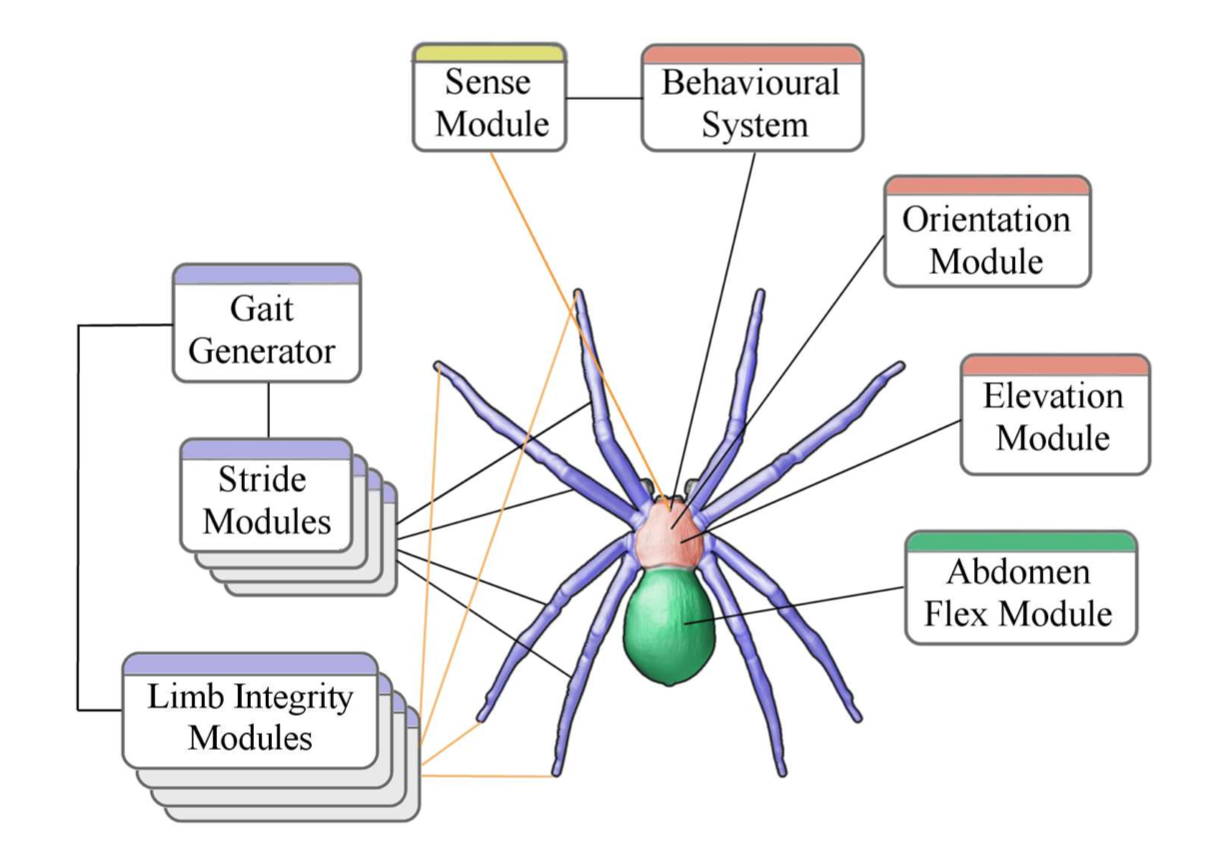
\includegraphics[height=8 cm]{figures/spider_module.png}
\caption{Main components of the arthropod animation system. \protect\cite{thesis}}
\label{fig:spider_module}
\end{figure}.
The schema of the system is based on the three locomotion layers which originally proposed in \cite{steering}. The three locomotion layers are action selection, steering and locomotion layer. The action selection is to choose which kind of behavior intend to animate which could be random stop, wander. The steering behavior is how the object move without consideration of the details of the locomotion. The locomotion layer is actually how to move the limbs given a specific steering behavior. 
\begin{figure}[ht!]
\centering
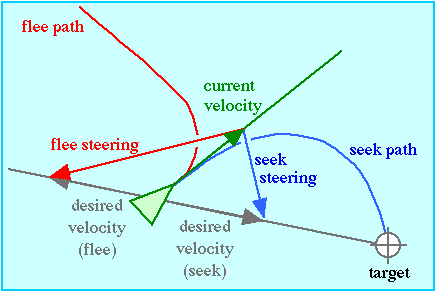
\includegraphics[height=6cm]{figures/seek.png}
\caption{Seek and flee steering diagram. \protect\cite{steeringImage}}
\label{fig:seek}
\end{figure}
The behavior system is corresponding to the action selection layer and the steering layer in \cite{steering}. An example of seek and flee action along with its steering details is shown in figure \ref{fig:seek}. The behavior system in \cite{thesis} mainly describes the kinematics of the spider without much consideration of limbs. Thus it introduce an abstract separation between the main body and limbs. The basics of the behavior system is meant to implement several behaviors such as wander, seek and flee by using physics and configuration which include such as the maximum speed of the spider, the maximum DOF of the joint between abdomen and thorax.
The rest of the system is mainly corresponding to the locomotion layer in \cite{steering}.
The major modules in the locomotion layer involve IK, stride module, limb regulatory modules, elevation and orientation module, abdominal flexing and the sense module. The examples of spider with IK is shown in \ref{fig:spiderIK}.
\begin{figure}[ht!]
\centering
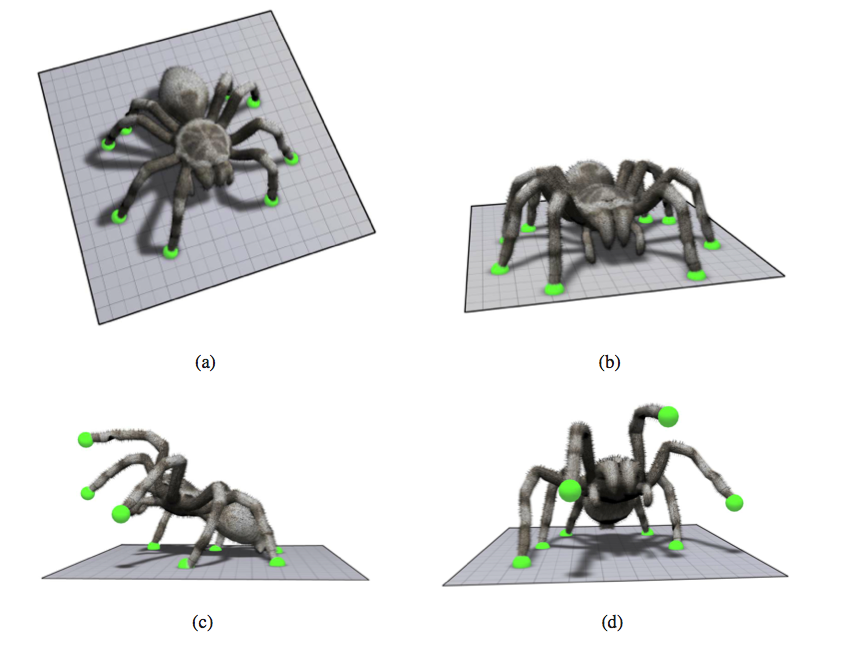
\includegraphics[height=10cm]{figures/spiderIK.png}
\caption{Results of spider with IK. \protect\cite{thesis}}
\label{fig:spiderIK}
\end{figure}
The main aim of the stride module is acting as a procedural step which move the creature's foot from initial to goal position. Results on the trajectory produced by the stride module is shown in figure \ref{fig:stride}.
\begin{figure}[ht!]
\centering
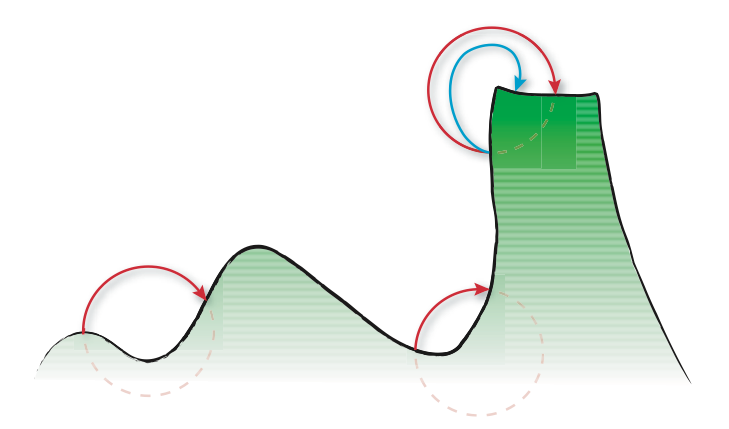
\includegraphics[height=6cm]{figures/stride.png}
\caption{Step path produced by the stride module. \protect\cite{thesis}}
\label{fig:stride}
\end{figure}
The limb regulatory modules act as an error checking function when an error in the limb is detected, the
gait generator will be invoked to correct a step. The gait pattern adopts the tripod trait. 
The purpose of the elevation and orientation modules is to control the absolute
orientation and the height of the main body which is the creature's
thorax and abdomen segments so that it conforms to a natural posture
relative to the position of the creature's feet. The function of abdominal flexing
is similar to limb regulatory module which is give constraints to the
joint which connects the thorax and the abdomen to make the posture
more natural. 
There are also two other modules. The sense module and the gravity activation.
The sense module acts as the eye of the creature which implemented mainly by the technique ray tracing but also take consideration of the limbs' feedback. The gravity module is added last to tackle the problem of special cases such as lose grip. The gravity activation is added last since it won't interfere the creature's normal locomotion since the mass of the creature is light and this choice will save lots of unnecessary constraints of the physical model\cite{thesis}.
\section{Arthropod Rendering}
The general technique to render an arthropod is texture mapping
which is a method for adding detail, surface texture or color to a 3D
model. For example, the surface of an arthropod could be added to the
mesh model to make the arthropod more realistic. Since the surface of the
arthropod is not smoothing, a bump mapping texture could be used to
show the indents in the surface. 
However, it is not enough. Because it is infeasible to use just
texture mapping to show the subtle detail of a
spider such as the fur of a spider. 
A common approach used is to use polygon strip fur which is produced
from side-view texture maps \cite{fur} as shown in figure \ref{fig:fur}.
\begin{figure}[ht!]
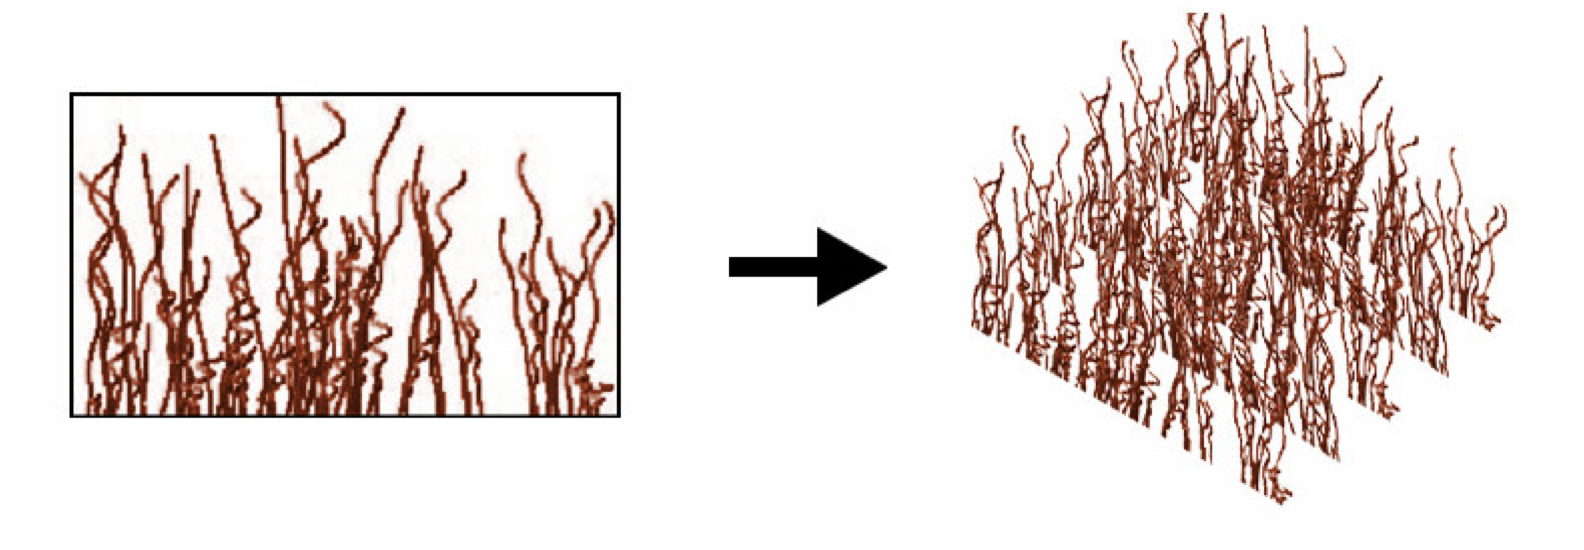
\includegraphics[height=5 cm]{figures/fur.png}
\caption{Polygon strip fur \protect\cite{fur}}
\label{fig:fur}
\end{figure}
The drawback of this approach is that if the fur is viewed from
side-view angle or directly above, it will not be rendered. However
this could be solved either in a 'cross-hatching' approach which is
strips are arranged at various angles across the skin surface or a
'Billboarding' approach which rotates any given polygon given strip to
always face to the camera \cite{fur}.
The most popular to generate fur
of an arthropod is the fins and shells approach. The fins technique 
involves the creation of textured polygon strips along the edges of
the base model and the fins extruded by default along the normal of
each edge \cite{thesis}.  The stages of fins application over a spider
is shown in \ref{fig:fins}.
\begin{figure}[ht!]
\centering
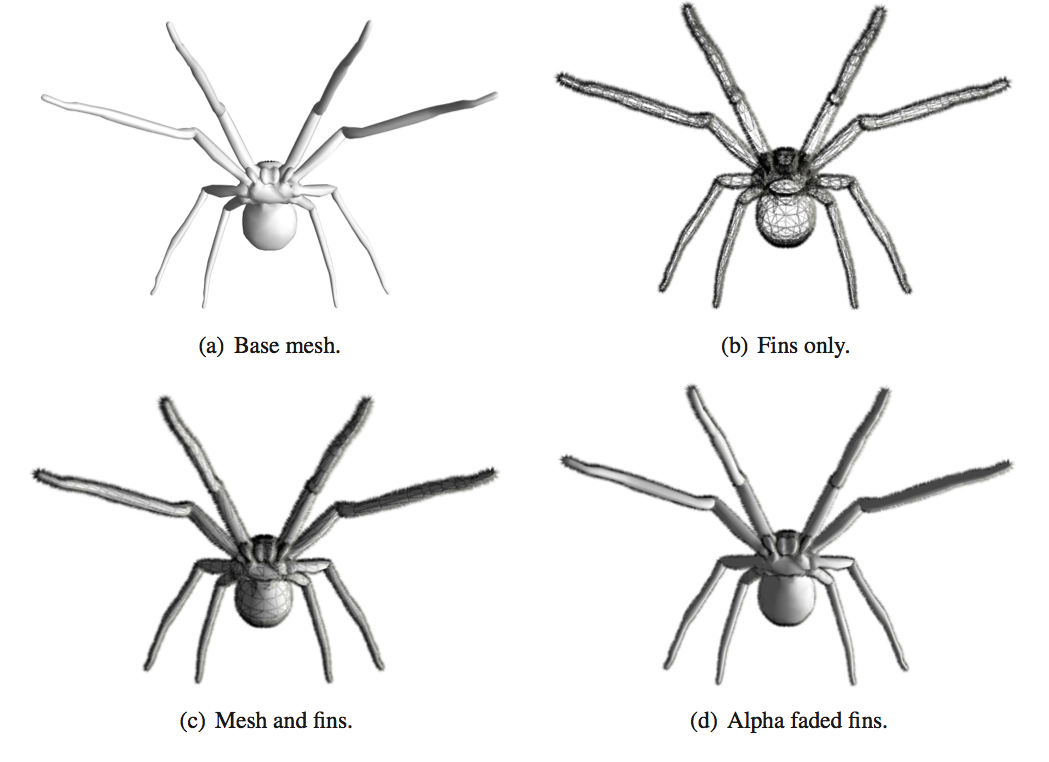
\includegraphics[height=12 cm]{figures/fins.png}
\caption{stages of fins \protect\cite{thesis}}
\label{fig:fins}
\end{figure}
The basic premise behind shells is adopting the texels approach with
traditional texturing methods to render a series of layers on which
cross-sections of a fur patch are rendered\cite{thesis}.
In sum, the polygon strip techniques could produce deserved
results. However there are drawbacks in it. The 'cross-hatching' will
result in slow rendering time for complex geometry. The bill boarding
approach does not have this problem but can not be viewed from
directly above. The fins and shells approach is usually more efficient
than polygon strip model and only major restriction is the maximum
DOF of the fur is 45$^\circ$ \cite{fur}.

